\documentclass[article]{jss}\usepackage[]{graphicx}\usepackage[]{color}
% maxwidth is the original width if it is less than linewidth
% otherwise use linewidth (to make sure the graphics do not exceed the margin)
\makeatletter
\def\maxwidth{ %
  \ifdim\Gin@nat@width>\linewidth
    \linewidth
  \else
    \Gin@nat@width
  \fi
}
\makeatother

\definecolor{fgcolor}{rgb}{0.345, 0.345, 0.345}
\newcommand{\hlnum}[1]{\textcolor[rgb]{0.686,0.059,0.569}{#1}}%
\newcommand{\hlstr}[1]{\textcolor[rgb]{0.192,0.494,0.8}{#1}}%
\newcommand{\hlcom}[1]{\textcolor[rgb]{0.678,0.584,0.686}{\textit{#1}}}%
\newcommand{\hlopt}[1]{\textcolor[rgb]{0,0,0}{#1}}%
\newcommand{\hlstd}[1]{\textcolor[rgb]{0.345,0.345,0.345}{#1}}%
\newcommand{\hlkwa}[1]{\textcolor[rgb]{0.161,0.373,0.58}{\textbf{#1}}}%
\newcommand{\hlkwb}[1]{\textcolor[rgb]{0.69,0.353,0.396}{#1}}%
\newcommand{\hlkwc}[1]{\textcolor[rgb]{0.333,0.667,0.333}{#1}}%
\newcommand{\hlkwd}[1]{\textcolor[rgb]{0.737,0.353,0.396}{\textbf{#1}}}%
\let\hlipl\hlkwb

\usepackage{framed}
\makeatletter
\newenvironment{kframe}{%
 \def\at@end@of@kframe{}%
 \ifinner\ifhmode%
  \def\at@end@of@kframe{\end{minipage}}%
  \begin{minipage}{\columnwidth}%
 \fi\fi%
 \def\FrameCommand##1{\hskip\@totalleftmargin \hskip-\fboxsep
 \colorbox{shadecolor}{##1}\hskip-\fboxsep
     % There is no \\@totalrightmargin, so:
     \hskip-\linewidth \hskip-\@totalleftmargin \hskip\columnwidth}%
 \MakeFramed {\advance\hsize-\width
   \@totalleftmargin\z@ \linewidth\hsize
   \@setminipage}}%
 {\par\unskip\endMakeFramed%
 \at@end@of@kframe}
\makeatother

\definecolor{shadecolor}{rgb}{.97, .97, .97}
\definecolor{messagecolor}{rgb}{0, 0, 0}
\definecolor{warningcolor}{rgb}{1, 0, 1}
\definecolor{errorcolor}{rgb}{1, 0, 0}
\newenvironment{knitrout}{}{} % an empty environment to be redefined in TeX

\usepackage{alltt}

%% -- LaTeX packages and custom commands ---------------------------------------

%% recommended packages
\usepackage{thumbpdf,lmodern}
\usepackage{float,tikz}
%% another package (only for this demo article)
\usepackage{framed}
%% author pakckage
\usepackage{xcolor,caption, float}

\graphicspath{ {./imgs/} }

%% new custom commands
\newcommand{\class}[1]{`\code{#1}'}
\newcommand{\fct}[1]{\code{#1()}}

% <<preliminaries, echo=FALSE, results=hide>>=


%% -- Article metainformation (author, title, ...) -----------------------------

%% - \author{} with primary affiliation
%% - \Plainauthor{} without affiliations
%% - Separate authors by \And or \AND (in \author) or by comma (in \Plainauthor).
%% - \AND starts a new line, \And does not.
\author{Thomas Huet\\UMR 5140}
%   \And Second Author\\Plus Affiliation}
\Plainauthor{Thomas Huet}

%% - \title{} in title case
%% - \Plaintitle{} without LaTeX markup (if any)
%% - \Shorttitle{} with LaTeX markup (if any), used as running title
\title{Modelling Prehistorical Iconographic Compositions. The \proglang{R} package \pkg{decorr}}
\Plaintitle{Modelling Prehistorical Iconographic Compositions. The R package 'decorr'}
\Shorttitle{Modelling Prehistorical Iconographic Compositions}

%% - \Abstract{} almost as usual
\Abstract{
  By definition, Prehistorical societies are characterised by the absence of a writing system. Prehistorical times cover more than 99\% of the human living. Even if it is being discussed, first symbolic manifestations start around 200,000 BC \citep{dErrico00}. The duration from first symbolic expressions to start of writing represents 97\% of the human living. In illiterate societies, testimonies of symbolic systems mostly come from iconography (ceramic decorations, rock-art, statuary, etc.) and signs are displayed mostlty a discontinuous figures which can have different relationships one with another. An graphical composition can be "read" as a spatial distribution of features having intrinsic values possibily having meaningful relationships one with another depending on their pairwise spatial proximities. 

  To understand meaningful associations of signs, geometric tools, graph analysis and statistical analysis offer great tools to recognize iconographical patterns and to infer collective conventions. We present the \pkg{decorr} \proglang{R} package which ground concepts, methods and tools to analyse ancient graphical systems.
}

\Keywords{Iconography, Prehistory, Graph Theory, Graph Drawing, Spatial Analysis, \proglang{R}}
\Plainkeywords{Iconography, Prehistory, Graph Theory, Graph Drawing, Spatial Analysis, R}

\Address{
  Thomas Huet\\
  CNRS-UMR 5140 \\
  Archeologie des Societes Mediterraneennes\\
  Universite Paul Valery\\
  route de Mende\\
  Montpellier 34199, France\\
  E-mail: \email{thomashuet7@gmail.com}\\
%  URL: \url{https://eeecon.uibk.ac.at/~zeileis/}
}
\IfFileExists{upquote.sty}{\usepackage{upquote}}{}
\begin{document}
% \Sweave2knitr("article_rvTH14_1.Rnw")
\SweaveOpts{concordance=TRUE}

\section[Introduction]{Introduction} \label{sec:intro}

For decades, study of ancient iconography was linked to history of religion because closely linked to symbolism, believes and religions. Since the \textit{New Archaeology} developpement during the 60's \citep{Clarke14}, symbolic expressions start to be studied with the same formal methods (statistics, seriations, distribution maps, etc.) as any another aspect of social organisation: settlement patterns, tools \emph{chaine opératoire}, susbsitence strategies, etc. \citep{Renfrew91}, \citep{LeroiGourhan92}. But unlike many aspects of the material culture -- a flint blade for cutting, a pottery for containing, a house for living --, the function of an iconographic composition cannot be drawn directly from itself. Whether study of ancient iconography had  undergone significative improvements at the site scale -- with GIS, database, paleoclimatic restitutions, etc. -- and at the sign scale with the development of archaeological sciences -- radiocarbon dating, use-wear analysis, elemental analysis, etc. --, these improvement do not necessarly help to understand the semantic content of the iconography.
Semantics or semiotics can be defined as a system of conventional signs organised also in conventional manners.  
Until our days, formal methods to study ancient iconography Semantics, has been mostlty been grounded (explicitly or not) on the prime principle of Saussurian linguistic: the 'linearity of the signifier' \citep{Saussure89}.  
Writing is one of the most rational semiographical system. With a clear distinction between signified and signifier -- specially in alphabetic and binary writings -- and the development of the signified on a horizontal, vertical or boustrophedon axis. 
Let us take the example of the word "\code{art}" which contains three vertices (\code{a}, \code{r}, \code{t}) and two edges (one between \code{a} and \code{r}, the other between \code{r} and \code{t}). In \proglang{R}, these features, concatenated in this order with a \code{paste0()}, is \code{art}, and not \code{rat}

% \SweaveOpts{width=3,height=1}
\begin{figure}[H]
\begin{knitrout}
\definecolor{shadecolor}{rgb}{0.969, 0.969, 0.969}\color{fgcolor}

\includegraphics[width=\maxwidth]{figure/unnamed-chunk-1-1} 

\end{knitrout}
\captionof{figure}[directional links]{concatenate of \code{a}, \code{r} and \code{t} graphical units (GUs) is \code{art}.}
\end{figure}

But, as stated, in Prehistorical the writing system does not exists. Spatial relationships between graphical features, or graphical units (GUs) are not necessarly linear and directed but could most probably be more multi-directional and undirected: the direction of the interactions of pairwise GUs can be in any order.  

\begin{figure}[H]
\begin{knitrout}
\definecolor{shadecolor}{rgb}{0.969, 0.969, 0.969}\color{fgcolor}
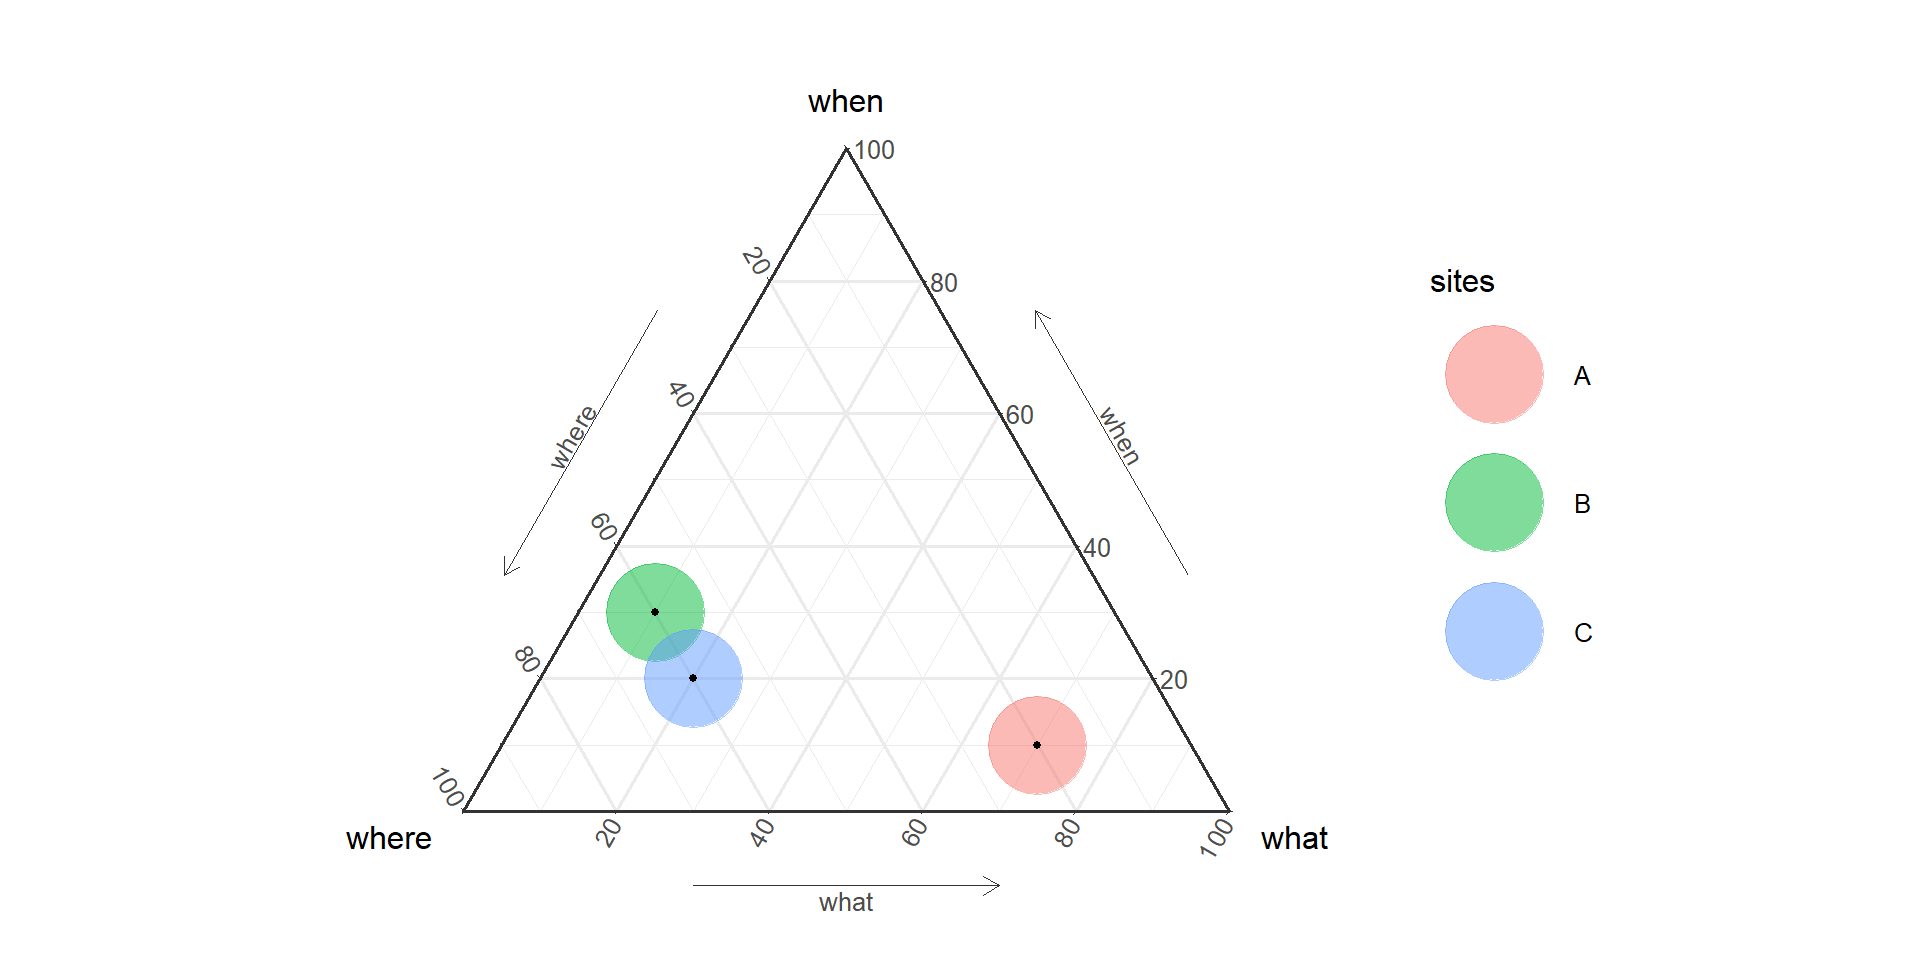
\includegraphics[width=\maxwidth]{figure/unnamed-chunk-2-1} 

\end{knitrout}
\captionof{figure}[multidirectional links]{Potential spatial relations between \code{a}, \code{r} and \code{t} GUs.}
\end{figure}

Applying the Saussurian model to any prehistorical graphical content had led to tedious division of the iconographical content with, for example, graphical as a relationship of \emp{figures} grouping GUs, \emp{patterns} grouping \emp{figures}, \emp{motives} grouping \emp{patterns}, etc., until the entire decorated support is described and can be compared to another decoration (XXX). But during this \emph{decomposition} process, many imprecisions occur:
\begin{itemize}
  \item groups and relationships are often defined empirically
  \item their level of significance are often implicit 
  \item the iconographical and spatial proximities between GUs and categories of GUs are not quantified
\end{itemize}

Furthermore, due to the inherent variability of iconography, most of the studies developp proper descriptive vocabularies, singular relationships of categories, idosyncratic methods in a site-dependend or period-dependend scales. This limits drastically the possibility to conduct cross-cultural comparisons and to draw a synthesis of humankind's symbolism at a large scale and over the long-term. 
\\
\\
In this article we present the \proglang{R} package \pkg{decorr}. Its purpose is to formalise a method based on geometric graphs to analyse any graphical content. As any formal system, iconography can be modelled as spatial features related one with the other depending on rules of spatial proximities. The idea is that a graphical system can be represented by vertices connected (or not) to each other with edges. This package has been grounded on the seminal work of C. Alexander \citep{Alexander08} and its first IT implementation by T. Huet \citep{Huet18a}. 

\section[Model]{Model} \label{sec:model}

Graph theory offers a conceptual framework and indices (global at the entire graph scale, local at the vertex scale) to deal with notions of networks, relationships and neighbourhoods. The spatial levels of the GUs can be retrieve by a planar graph (Graph Theory) and a spatial (GIS) analysis.
Nodes and edges -- repectively for GUs and their connexion -- are created on a GIS interface. 
In the GIS, the decoration figure is open in the first place in a new project with no projection. The decoration image will be considerated as the basemap of the project and will cover the region of interest of the analysis. The decoration image can be binarized where GUs are considerated active and the undecorated parts of the support, or background, are considerated inactive. After what, the decoration image is tiled. A simplier solution will be to create directly centroids over the GUs. The \emph{x} and \emph{y} coordinates of the nodes are relative to the decoration and measured in pixels.
Exist a link between a couple of GUs when these graphical units share a border. A planar graph is constructed from grahical units (nodes) and their proximity links (edges). This model is a Voronoi diagram of the support where the Voronoi seeds are the GUs. Its geographical equivalent is a Thiessen polygon.


\begin{figure}[H]
\centering
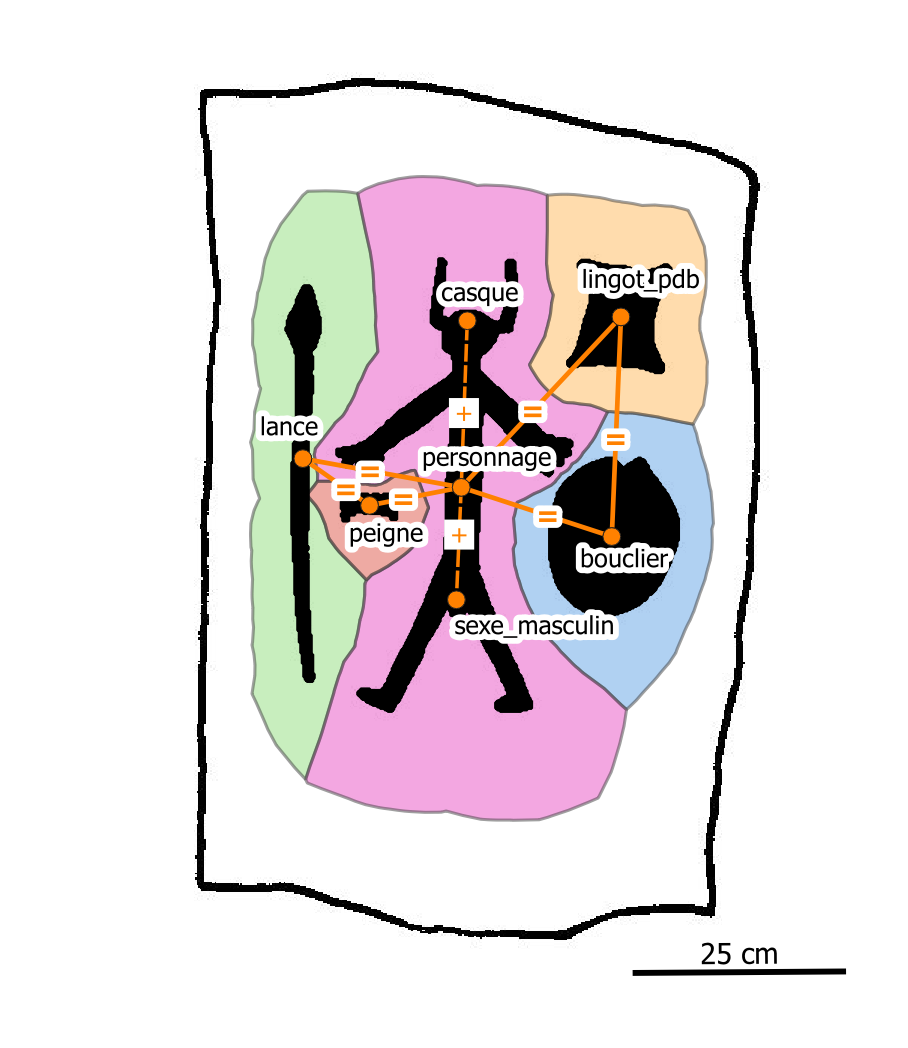
\includegraphics{gis}
\caption{\label{fig:gis} GIS interface. A) Original decoration of the Late Bronze Age \emp{Cerro Muriano 1} stele (drawing: \cite{DiazGuardamino10}) with its extent (\code{xmin, xmax, ymin, ymax}); B) After the polygonisation of the GUs, including the border of the stelae, the Voronoi cells, the centroid of GUs and the links between GUs having adjacent cells (ie, sharing a border) are calculated; C) For each GUs, \emph{x} and \emph{y} are calculated; D) At least one variable, like the \code{type} of the GUs is defined in order to compute composition analysis.}
\end{figure}

This model has a minimal of \emph{a priori} definitions. Those definitions only concern the GUs (type, technology, color, orientation, size, etc.). The plasticity of fraph theory allows to develop conventions in order to quote the different types of relations between GUs.\\

By convention, two different GUs having a Voronoi cell sharing a border, have an edge tagged \code{'='} and represented with a plain line. The textual notation of a such edge is \code{'-=-'}. For example: \code{1 -=- 4} means that the nodes \code{1} and \code{4} have a common border.

But it occurs frequently that a GU can be divided into a \emph{main unit} (eg, a character) and one or various \emph{attribute units} (eg, a helmet, male sex). To record this information, a new type of edge, tagged with \code{'+'}, is be introduced. This type of edges is be directed and displayed with a dashed line. Its starts from the \emph{main unit} and ends with the \emph{attribute units}. For example \code{4 -+- 6}) means that the main node \code{4} has the attribute node \code{6}.

\begin{figure}[H] 
\centering
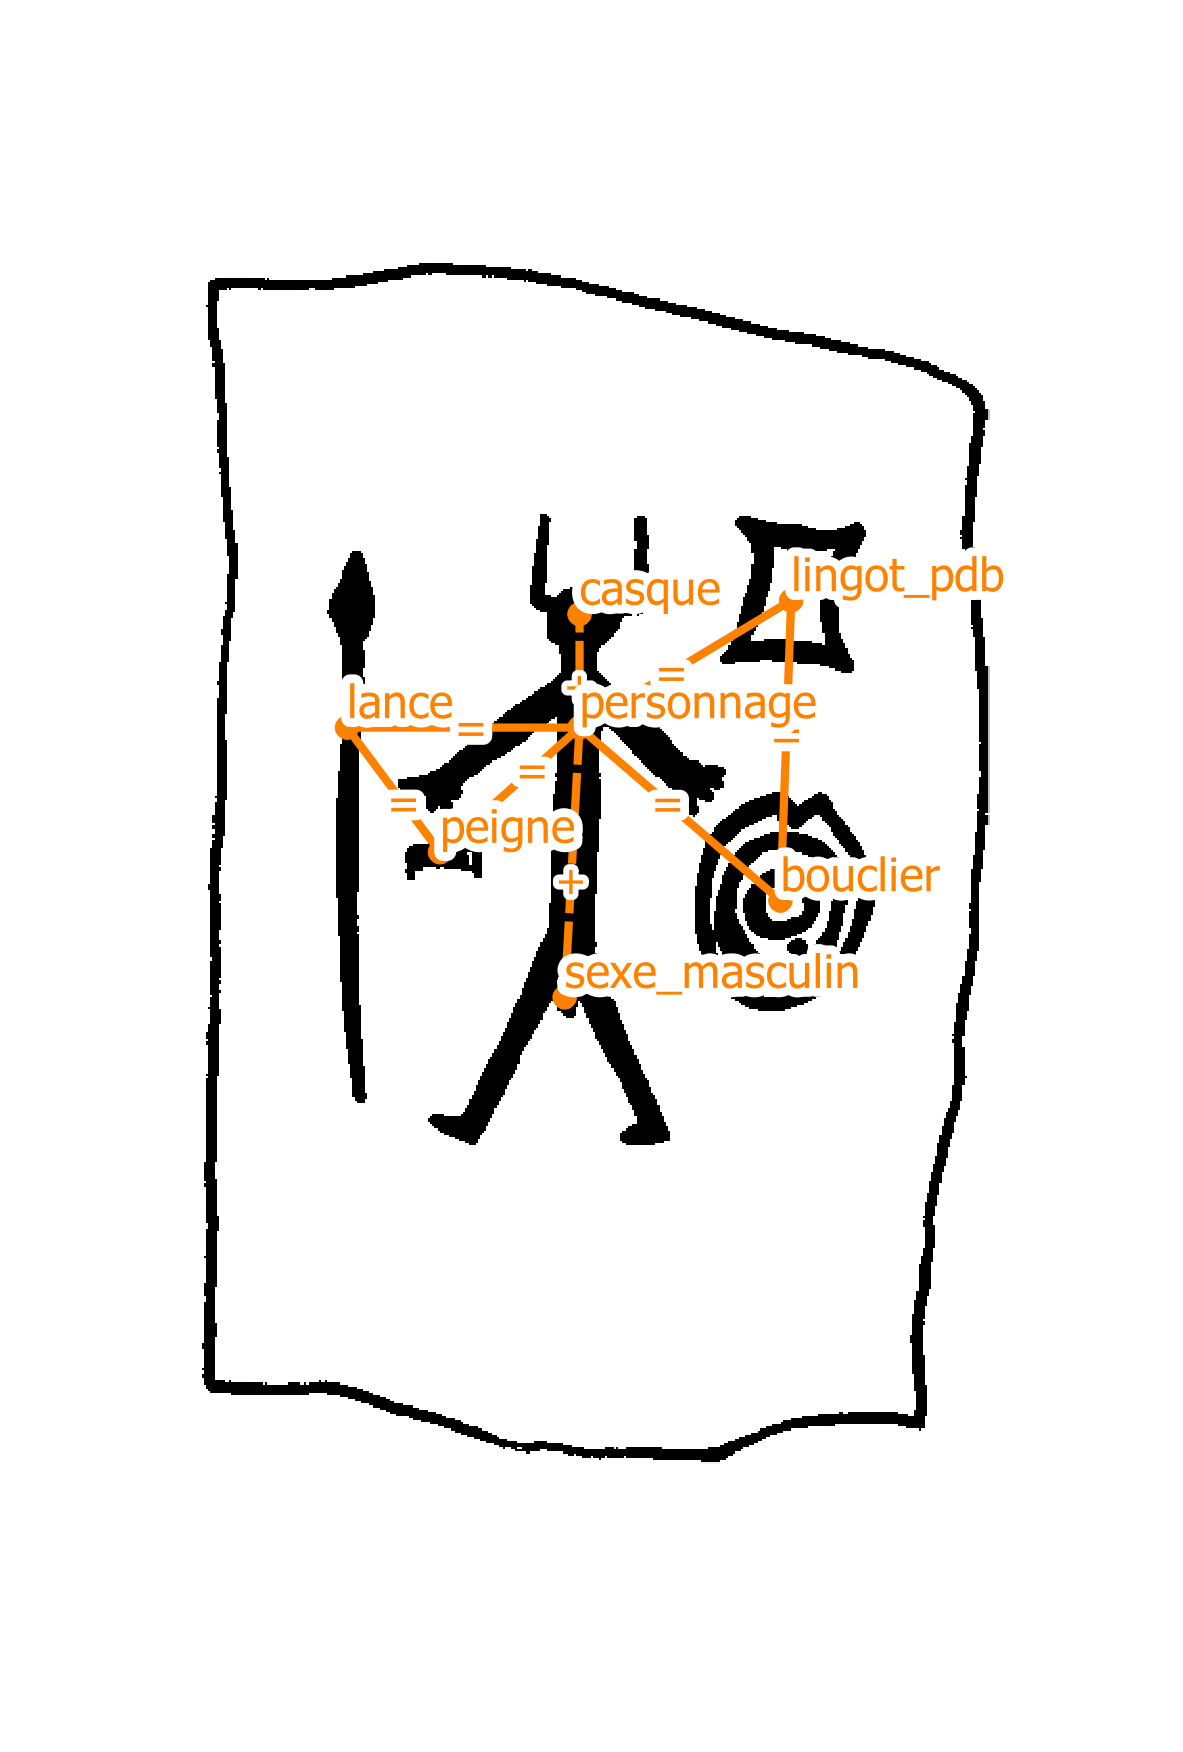
\includegraphics[scale=0.3]{gis_1}
\caption{\label{fig:gis1} GIS interface. The GUs 'casque' (helmet) and 'sexe\_masculin' (male sex) are two attributes of the GU 'personnage' (character).}
\end{figure}

Finally, it is quite common that a graphical composition shows superimpositions between different UGs. This stratigraphic information (\code{A} \emph{over} \code{B}, or \code{B} \emph{under} \code{A}) helps to understand the relative chronology between GUs and must be recorded. A simple way to achieve this is to introduce the new tag \code{'>'} for the for the type of edge. This type of edges is directed. For example \code{A ->- B} means that \code{A} crosses \code{B}. 


\begin{table}[H]
% \begin{center}
  \centering
 \begin{tabular}{|p{.5cm} p{.5cm} p{.5cm} p{2cm} p{2cm} p{5cm}|}
 \hline
  % node A & type of edge & node B & undirected & birel & stratigraphical meaning \\
 node 1 & edge type & node 2 & (un)directed & \emph{birel} & stratigraphical meaning \\
 \hline
  \code{A} & \code{=} & \code{B} & undirected & $ A \cap B = \emptyset $ & \code{A} and \code{B} are disjoint, \code{A} and \code{B} can be contemporaneous \\
  \code{A} & \code{+} & \code{B} & directed & $ A \cap B = A $ & \code{A} and \code{B} are contemporaneous, \code{B} is an attribute of \code{A} \\
  \code{A} & \code{>} & \code{B} & directed & $ A \cap B = \exists $ & \code{A} overlaps \code{B}, \code{A} can be more recent than \code{B} \\
 % \code{1} & = & 2 & undirected & A \cap B = \varnothing & 1 and 2 can be contemporaneous \\
 \hline
\end{tabular}
\caption{Synthesis for the different types of relations between GUs}\label{tab1}
% \end{center}
\end{table}

\section{The R package decorr} \label{sec:models}

The \pkg{decorr} package can be downloaded from GitHub
%
\begin{CodeChunk}
\begin{CodeInput}
R>   devtools::install_github("zoometh/iconr")
\end{CodeInput}
\end{CodeChunk}
%

\subsection{External package} \label{sec:ext_pck}

The \pkg{decorr} package imports the following packages:
\begin{itemize}
\setlength\itemsep{.1em}
  \item \pkg{magick} for image manipulation \citep{Ooms18}
  \item \pkg{igraph} for graph and network analysis \citep{Csardi06} 
  \item \pkg{rgdal}  to read shapefiles of nodes and/or edges \citep{Bivand19}
  \item \pkg{grDevices} for colors and font plotting, \pkg{graphics} for graphics, \pkg{utils} and \pkg{methods} for formally defined methods and \emph{varia} methods (all combinations, etc.) \citep{R19}
\end{itemize}

\subsection{Data} \label{sec:ext_data}

The training dataset is a selection of four drawing of stelae belonging to the Late Bronze age of the SW Iberian peninsula. At the first, the training dataset is in the \code{extdata} folder of the \pkg{decorr}. The dataframe storing the inventory of decorations is \code{imgs}.

\begin{itemize}
\item The \code{imgs} dataframe structure is
\end{itemize}

% latex table generated in R 3.6.1 by xtable 1.8-4 package
% Thu Sep 24 12:13:36 2020
\begin{table}[ht]
\centering
\begin{tabular}{rlll}
  \hline
idf & site & decor & img \\ 
  \hline
  1 & Cerro Muriano & Cerro Muriano 1 & Cerro\_Muriano.Cerro\_Muriano\_1.jpg \\ 
    2 & Torrejon Rubio & Torrejon Rubio 1 & Torrejon\_Rubio.Torrejon\_Rubio\_1.jpg \\ 
    3 & Brozas & Brozas & Brozas.Brozas.jpg \\ 
    4 & Zarza de Montanchez & Zarza De Montanchez & Zarza\_de\_Montanchez.Zarza\_De\_Montanchez.jpg \\ 
   \hline
\end{tabular}
\caption{The studied corpus, the imgs.tsv dataframe} 
\label{Test_table}
\end{table}


The field \code{imgs$idf} is the short name of the decoration, useful during statistical analysis. The primary key of each decoration is the concatenate of \code{imgs$site} and \code{imgs$decor}.\\

At first the drawing dataset can be checked by using the \code{imgs} dataframe and the \pkg{magick}

\SweaveOpts{width=16,height=16}
\begin{figure}[H]
\begin{knitrout}
\definecolor{shadecolor}{rgb}{0.969, 0.969, 0.969}\color{fgcolor}\begin{kframe}
\begin{alltt}
\hlkwd{library}\hlstd{(magick)}
\end{alltt}


{\ttfamily\noindent\color{warningcolor}{\#\# Warning: package 'magick' was built under R version 3.6.3}}

{\ttfamily\noindent\itshape\color{messagecolor}{\#\# Linking to ImageMagick 6.9.9.14\\\#\# Enabled features: cairo, freetype, fftw, ghostscript, lcms, pango, rsvg, webp\\\#\# Disabled features: fontconfig, x11}}\begin{alltt}
\hlstd{pth} \hlkwb{<-} \hlkwd{system.file}\hlstd{(}\hlstr{"extdata"}\hlstd{,} \hlkwc{package} \hlstd{=} \hlstr{"decorr"}\hlstd{)}
\hlstd{imgs} \hlkwb{<-} \hlkwd{read.table}\hlstd{(}\hlkwd{system.file}\hlstd{(}\hlstr{"extdata"}\hlstd{,} \hlstr{"imgs.tsv"}\hlstd{,} \hlkwc{package} \hlstd{=} \hlstr{"decorr"}\hlstd{),}
                      \hlkwc{sep}\hlstd{=}\hlstr{"\textbackslash{}t"}\hlstd{,} \hlkwc{stringsAsFactors} \hlstd{=} \hlnum{FALSE}\hlstd{)}
\hlstd{lims} \hlkwb{<-} \hlkwd{list}\hlstd{()}
\hlkwa{for}\hlstd{(i} \hlkwa{in} \hlnum{1}\hlopt{:}\hlkwd{nrow}\hlstd{(imgs))\{}
  \hlstd{i1} \hlkwb{<-} \hlkwd{image_read}\hlstd{(}\hlkwd{paste0}\hlstd{(pth,}\hlstr{"\textbackslash{}\textbackslash{}"}\hlstd{,imgs[i,}\hlstr{"img"}\hlstd{]))}
  \hlstd{lbl.txt} \hlkwb{<-} \hlkwd{paste0}\hlstd{(imgs[i,}\hlstr{"idf"}\hlstd{],}\hlstr{"\textbackslash{}n"}\hlstd{,}
                    \hlstd{imgs[i,}\hlstr{"site"}\hlstd{],}\hlstr{"\textbackslash{}n"}\hlstd{,}
                    \hlstd{imgs[i,}\hlstr{"decor"}\hlstd{],}\hlstr{"\textbackslash{}n"}\hlstd{,}
                    \hlstd{imgs[i,}\hlstr{"img"}\hlstd{],}\hlstr{"\textbackslash{}n"}\hlstd{,}
                    \hlkwd{image_info}\hlstd{(i1)}\hlopt{$}\hlstd{width,}\hlstr{"*"}\hlstd{,}\hlkwd{image_info}\hlstd{(i1)}\hlopt{$}\hlstd{height,}\hlstr{" px"}\hlstd{)}
  \hlstd{i1} \hlkwb{<-} \hlkwd{image_annotate}\hlstd{(i1,lbl.txt,}\hlkwc{location} \hlstd{=} \hlstr{"northwest"}\hlstd{,}
                       \hlkwc{size} \hlstd{=} \hlnum{25}\hlstd{,} \hlkwc{color} \hlstd{=} \hlstr{"red"}\hlstd{)}
  \hlstd{lims[[}\hlkwd{length}\hlstd{(lims)}\hlopt{+}\hlnum{1}\hlstd{]]}\hlkwb{<-} \hlstd{i1}
\hlstd{\}}
\hlstd{out.img} \hlkwb{<-} \hlkwd{image_append}\hlstd{(}\hlkwd{c}\hlstd{(}\hlkwd{image_append}\hlstd{(}\hlkwd{c}\hlstd{(lims[[}\hlnum{1}\hlstd{]],lims[[}\hlnum{2}\hlstd{]])),}
                          \hlkwd{image_append}\hlstd{(}\hlkwd{c}\hlstd{(lims[[}\hlnum{3}\hlstd{]],lims[[}\hlnum{4}\hlstd{]]))),}
                        \hlkwc{stack} \hlstd{=} \hlnum{TRUE}\hlstd{)}
\hlkwd{plot}\hlstd{(out.img)}
\end{alltt}
\end{kframe}
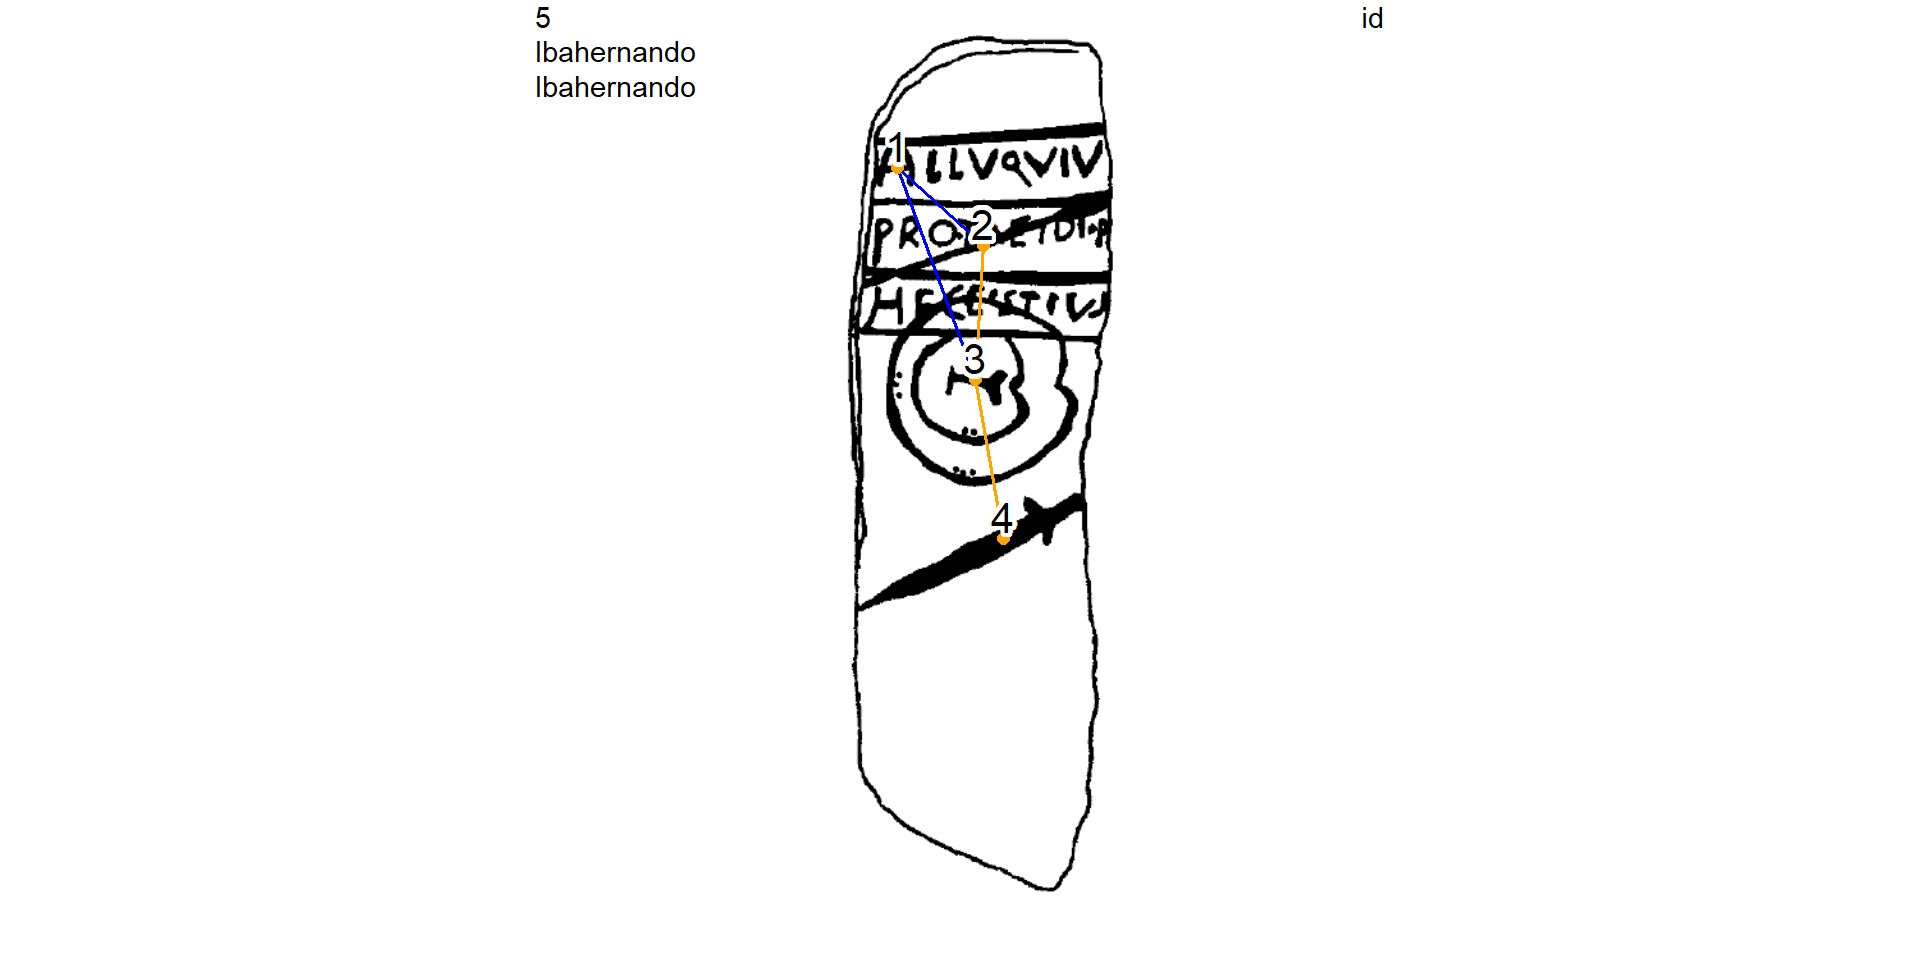
\includegraphics[width=\maxwidth]{figure/unnamed-chunk-4-1} 

\end{knitrout}
\captionof{figure}[directional links]{All decoration drawings belongs to \citep{DiazGuardamino10}}
\end{figure}

As said, the GIS offers the more suitable interface to register all GUs and to get their coordinates. But the coordinates origin (0,0) in a GIS is the bottom-left corner, while this origin is top-left for any \proglang{R} rasters or matrices: this will affect the \emph{y} axis. To recover the correct GUs coordinates on this axis, for nodes and edges, between the inputs in the GIS and the decoration image coordinates in \proglang{R}, the \pkg{decorr} calculate the absolute \emph{y} value and used the image height as a constant offset. 

To construct a graph overlapping the decoration images listed in the \code{images} dataframe, the first step is to load \code{nodes}, \code{edges} dataframes.

\begin{knitrout}
\definecolor{shadecolor}{rgb}{0.969, 0.969, 0.969}\color{fgcolor}\begin{kframe}
\begin{alltt}
\hlstd{nodes} \hlkwb{<-} \hlkwd{read.table}\hlstd{(}\hlkwd{system.file}\hlstd{(}\hlstr{"extdata"}\hlstd{,} \hlstr{"nodes.csv"}\hlstd{,} \hlkwc{package} \hlstd{=} \hlstr{"decorr"}\hlstd{),}
                    \hlkwc{sep}\hlstd{=}\hlstr{"\textbackslash{}t"}\hlstd{,}\hlkwc{stringsAsFactors} \hlstd{=} \hlnum{FALSE}\hlstd{)}
\hlstd{edges} \hlkwb{<-} \hlkwd{read.table}\hlstd{(}\hlkwd{system.file}\hlstd{(}\hlstr{"extdata"}\hlstd{,} \hlstr{"edges.csv"}\hlstd{,} \hlkwc{package} \hlstd{=} \hlstr{"decorr"}\hlstd{),}
                    \hlkwc{sep}\hlstd{=}\hlstr{"\textbackslash{}t"}\hlstd{,}\hlkwc{stringsAsFactors} \hlstd{=} \hlnum{FALSE}\hlstd{)}
\end{alltt}
\end{kframe}
\end{knitrout}

\begin{itemize}
\item The \code{nodes} dataframe structure is
\end{itemize}

\begin{kframe}
\begin{alltt}
\hlstd{nodes.cm} \hlkwb{<-} \hlkwd{subset}\hlstd{(nodes, decor} \hlopt{==} \hlstr{"Cerro Muriano 1"}\hlstd{)}
\hlstd{caption} \hlkwb{<-} \hlstr{"Nodes (\textbackslash{}\textbackslash{}code\{nodes.csv\} dataframe) for \textbackslash{}\textbackslash{}emph\{Cerro Muriano 1\}"}
\hlstd{xtable}\hlopt{::}\hlkwd{xtable}\hlstd{(nodes.cm,}
       \hlkwc{caption} \hlstd{= caption)}
\end{alltt}
\end{kframe}% latex table generated in R 3.6.1 by xtable 1.8-4 package
% Thu Sep 24 12:13:37 2020
\begin{table}[ht]
\centering
\begin{tabular}{rllrlrr}
  \hline
 & site & decor & id & type & x & y \\ 
  \hline
1 & Cerro Muriano & Cerro Muriano 1 &   1 & personnage & 349.81 & -298.32 \\ 
  2 & Cerro Muriano & Cerro Muriano 1 &   2 & casque & 349.81 & -243.99 \\ 
  3 & Cerro Muriano & Cerro Muriano 1 &   3 & lance & 238.46 & -298.32 \\ 
  4 & Cerro Muriano & Cerro Muriano 1 &   4 & bouclier & 446.02 & -381.17 \\ 
  5 & Cerro Muriano & Cerro Muriano 1 &   5 & peigne & 283.00 & -358.01 \\ 
  6 & Cerro Muriano & Cerro Muriano 1 &   7 & sexe\_masculin & 342.69 & -427.49 \\ 
  7 & Cerro Muriano & Cerro Muriano 1 &   8 & lingot\_pdb & 451.15 & -237.48 \\ 
   \hline
\end{tabular}
\caption{Nodes (\code{nodes.csv} dataframe) for \emph{Cerro Muriano 1}} 
\end{table}


\begin{itemize}
\item The \code{edges} dataframe structure is
\end{itemize}

\begin{kframe}
\begin{alltt}
\hlstd{edges.cm} \hlkwb{<-} \hlkwd{subset}\hlstd{(edges, decor} \hlopt{==} \hlstr{"Cerro Muriano 1"}\hlstd{)}
\hlstd{caption} \hlkwb{<-} \hlstr{"Edges (\textbackslash{}\textbackslash{}code\{edges.csv\} dataframe) for \textbackslash{}\textbackslash{}emph\{Cerro Muriano 1\}"}
\hlstd{xtable}\hlopt{::}\hlkwd{xtable}\hlstd{(edges.cm,}
               \hlkwc{caption}\hlstd{=caption)}
\end{alltt}
\end{kframe}% latex table generated in R 3.6.1 by xtable 1.8-4 package
% Thu Sep 24 12:13:38 2020
\begin{table}[ht]
\centering
\begin{tabular}{rllrrl}
  \hline
 & site & decor & a & b & type \\ 
  \hline
1 & Cerro Muriano & Cerro Muriano 1 &   1 &   8 & = \\ 
  2 & Cerro Muriano & Cerro Muriano 1 &   4 &   8 & = \\ 
  3 & Cerro Muriano & Cerro Muriano 1 &   1 &   4 & = \\ 
  4 & Cerro Muriano & Cerro Muriano 1 &   1 &   5 & = \\ 
  5 & Cerro Muriano & Cerro Muriano 1 &   3 &   5 & = \\ 
  6 & Cerro Muriano & Cerro Muriano 1 &   1 &   2 & + \\ 
  7 & Cerro Muriano & Cerro Muriano 1 &   1 &   7 & + \\ 
  8 & Cerro Muriano & Cerro Muriano 1 &   3 &   1 & = \\ 
   \hline
\end{tabular}
\caption{Edges (\code{edges.csv} dataframe) for \emph{Cerro Muriano 1}} 
\end{table}


For edges, there is no need to get the coordinates of the starting point and the ending point. These coordinates can be calculated from the \code{nodes} dataframe. For example, the first edge of the \emph{Cerro Muriano 1} decoration connect the nodes \code{1} and \code{8}. A way to retrieve coordinates of these two nodes -- which are the two end points -- will be:

\begin{knitrout}
\definecolor{shadecolor}{rgb}{0.969, 0.969, 0.969}\color{fgcolor}\begin{kframe}
\begin{alltt}
\hlstd{cm.1} \hlkwb{<-} \hlkwd{subset}\hlstd{(nodes, decor} \hlopt{==} \hlstr{"Cerro Muriano 1"} \hlopt{&} \hlstd{id} \hlopt{==} \hlnum{1}\hlstd{)[,}\hlkwd{c}\hlstd{(}\hlstr{"x"}\hlstd{,}\hlstr{"y"}\hlstd{)]}
\hlstd{cm.8} \hlkwb{<-} \hlkwd{subset}\hlstd{(nodes, decor} \hlopt{==} \hlstr{"Cerro Muriano 1"} \hlopt{&} \hlstd{id} \hlopt{==} \hlnum{8}\hlstd{)[,}\hlkwd{c}\hlstd{(}\hlstr{"x"}\hlstd{,}\hlstr{"y"}\hlstd{)]}
\hlkwd{cat}\hlstd{(}\hlkwd{as.numeric}\hlstd{(cm.1),}\hlstr{";"}\hlstd{,}\hlkwd{as.numeric}\hlstd{(cm.8))}
\end{alltt}
\begin{verbatim}
## 349.8148 -298.3244 ; 451.1489 -237.4782
\end{verbatim}
\end{kframe}
\end{knitrout}

Once done, the list of graphs can be stored with the \code{list_dec()} function.

\subsection{\code{list\_dec()} function} \label{sec:funlistdec}

The \code{list\_dec()} function allows to store graphs for each decorations stored into \code{nodes}, \code{edges} and \code{images} dataframes and store the graphs in a list. The join between these dataframes is done on the two fields \code{site} and \code{decor}. The first graph of can be plotted

\begin{figure}[H]
% \SweaveOpts{width=2,height=2}
\begin{knitrout}
\definecolor{shadecolor}{rgb}{0.969, 0.969, 0.969}\color{fgcolor}\begin{kframe}
\begin{alltt}
\hlkwd{par}\hlstd{(}\hlkwc{mar}\hlstd{=}\hlkwd{c}\hlstd{(}\hlnum{0.1}\hlstd{,}\hlnum{0.1}\hlstd{,}\hlnum{0.1}\hlstd{,}\hlnum{0.1}\hlstd{) )}
\hlkwd{library}\hlstd{(decorr)}
\hlcom{# imgs <- read.table(system.file("extdata", "imgs.tsv", package = "decorr"),}
\hlcom{#                       sep="\textbackslash{}t", stringsAsFactors = FALSE)}
\hlcom{# nodes <- read.table(system.file("extdata", "nodes.csv", package = "decorr"),}
\hlcom{#                     sep="\textbackslash{}t",stringsAsFactors = FALSE)}
\hlcom{# edges <- read.table(system.file("extdata", "edges.csv", package = "decorr"),}
\hlcom{#                     sep="\textbackslash{}t",stringsAsFactors = FALSE)}
\hlstd{lgrph} \hlkwb{<-} \hlkwd{list_dec}\hlstd{(imgs,nodes,edges,}\hlkwc{var}\hlstd{=}\hlstr{"type"}\hlstd{)}
\hlkwd{plot}\hlstd{(lgrph[[}\hlnum{1}\hlstd{]],}
     \hlkwc{vertex.color} \hlstd{=} \hlstr{"orange"}\hlstd{,}
     \hlkwc{vertex.frame.color}\hlstd{=}\hlstr{"orange"}\hlstd{,}
     \hlkwc{vertex.label.color} \hlstd{=} \hlstr{"black"}\hlstd{,}
     \hlkwc{vertex.size} \hlstd{=} \hlnum{10}\hlstd{,}
     \hlkwc{vertex.label.cex} \hlstd{=}\hlnum{.7}\hlstd{,}
     \hlkwc{edge.color} \hlstd{=} \hlstr{"orange"}
     \hlcom{# vertex.label.family="Courier New"}
     \hlstd{)}
\end{alltt}
\end{kframe}
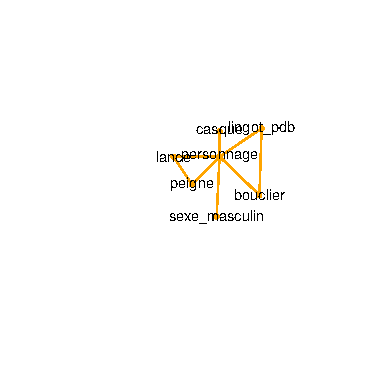
\includegraphics[width=\maxwidth]{figure/unnamed-chunk-8-1} 

\end{knitrout}
\captionof{figure}[directional links]{Plot of the first graph of the list}
\end{figure}

The others \pkg{decorr} package functions can be divided into:
\begin{enumerate}
 \item graphical functions
 \item single decoration functions
 \item comparisons between different decorations functions
\end{enumerate}

\subsection{Graphical functions} \label{sec:functions_gr}

The \pkg{decorr} has three purely graphical functions
\begin{itemize}
\setlength\itemsep{.1em}
\item \code{labels_shadow()} function is a re-use of the \code{shadowtext()} function from the \pkg{TeachingDemos} package \citep{Snow20}.
\item \code{side_plot_nds()} and \code{side_plot_eds()} allow to plot figures side-by-side for nodes or edges comparisons
\end{itemize}

\subsection{Single decoration functions} \label{sec:functions_one}

Functions allowing to create a geometric graph for a single decoration are:

\begin{itemize}
  \item \code{read_nds()} and \code{read_eds()} functions allow to read respectively a file of nodes and a file of edges (\code{.tsv} or \code{.shp} files)
\end{itemize}

The \code{read_nds()} function is close to the native \code{read.table()} function but allows to read \emph{shapefiles} of nodes.

the \code{read_eds()} permits to read a \emph{shapefiles} of nodes or to retrieve the coordinates of the ends of the edges from the \code{nodes} dataframe. For example, the first \emph{Torrejon Rubio 1} edge, between the nodes \code{6} and \code{5} has
the starting point (xa=366.7001, ya=-563.1358) and the ending point (xb=490.1195, yb=-513.2428)

\begin{figure}{H}
\centering
\begin{kframe}
\begin{alltt}
\hlcom{# library(decorr)}
\hlstd{sit} \hlkwb{<-} \hlstr{"Torrejon Rubio"} \hlstd{; dec} \hlkwb{<-} \hlstr{"Torrejon Rubio 1"}
\hlstd{nds.df} \hlkwb{<-} \hlkwd{read_nds}\hlstd{(}\hlkwc{site} \hlstd{= sit,} \hlkwc{decor} \hlstd{= dec,} \hlkwc{dev} \hlstd{=} \hlstr{".tsv"}\hlstd{,}
                   \hlkwc{doss} \hlstd{=} \hlkwd{system.file}\hlstd{(}\hlstr{"extdata"}\hlstd{,} \hlkwc{package} \hlstd{=} \hlstr{"decorr"}\hlstd{))}
\hlstd{eds.df} \hlkwb{<-} \hlkwd{read_eds}\hlstd{(}\hlkwc{site} \hlstd{= sit,} \hlkwc{decor} \hlstd{= dec,} \hlkwc{dev} \hlstd{=} \hlstr{".tsv"}\hlstd{,}
                   \hlkwc{doss} \hlstd{=} \hlkwd{system.file}\hlstd{(}\hlstr{"extdata"}\hlstd{,} \hlkwc{package} \hlstd{=} \hlstr{"decorr"}\hlstd{))}
\hlstd{xtable}\hlopt{::}\hlkwd{xtable}\hlstd{(eds.df[}\hlnum{1}\hlstd{,],}
               \hlkwc{caption}\hlstd{=}\hlstr{"first edge of the dataframe"}\hlstd{,}
               \hlkwc{label}\hlstd{=}\hlstr{"Test_table_1"}\hlstd{,}
               \hlkwc{size}\hlstd{=}\hlnum{7}\hlstd{)}
\end{alltt}
\end{kframe}% latex table generated in R 3.6.1 by xtable 1.8-4 package
% Thu Sep 24 12:13:38 2020
\begin{table}[ht]
\centering
\begin{tabular}{rllrrlrrrr}
  \hline
 & site & decor & a & b & type & xa & ya & xb & yb \\ 
  \hline
9 & Torrejon Rubio & Torrejon Rubio 1 &   6 &   5 & = & 366.70 & -563.14 & 490.12 & -513.24 \\ 
   \hline
\end{tabular}
\caption{first edge of the dataframe} 
\label{Test_table_1}
\end{table}

\end{figure}

\begin{itemize}
  \item \code{plot_dec_grph ()} allows to plot a geometric graph over a decoration image
\end{itemize}

Once, the imgs, nodes and edges dataframes have been read, the decoration graph is build and can be plotted, here for the \emph{Torrejon Rubio 1} decoration. The \code{lbl.txt} parameter allow to decide which field of the nodes will be displayed as the label, here the column \code{nodes$type}

\SweaveOpts{width=3,height=3}
\begin{figure}{H}
\centering
\begin{knitrout}
\definecolor{shadecolor}{rgb}{0.969, 0.969, 0.969}\color{fgcolor}\begin{kframe}
\begin{alltt}
\hlkwd{library}\hlstd{(decorr)}
\hlkwd{par}\hlstd{(}\hlkwc{mar}\hlstd{=}\hlkwd{c}\hlstd{(}\hlnum{1}\hlstd{,}\hlnum{1}\hlstd{,}\hlnum{1}\hlstd{,}\hlnum{1}\hlstd{) )}
\hlstd{sit} \hlkwb{<-} \hlstr{"Torrejon Rubio"} \hlstd{; dec} \hlkwb{<-} \hlstr{"Torrejon Rubio 1"}
\hlstd{nds.df} \hlkwb{<-} \hlkwd{read_nds}\hlstd{(}\hlkwc{site} \hlstd{= sit,} \hlkwc{decor} \hlstd{= dec,} \hlkwc{dev} \hlstd{=} \hlstr{".tsv"}\hlstd{,}
                   \hlkwc{doss} \hlstd{=} \hlkwd{system.file}\hlstd{(}\hlstr{"extdata"}\hlstd{,} \hlkwc{package} \hlstd{=} \hlstr{"decorr"}\hlstd{))}
\hlstd{eds.df} \hlkwb{<-} \hlkwd{read_eds}\hlstd{(}\hlkwc{site} \hlstd{= sit,} \hlkwc{decor} \hlstd{= dec,} \hlkwc{dev} \hlstd{=} \hlstr{".tsv"}\hlstd{,}
                   \hlkwc{doss} \hlstd{=} \hlkwd{system.file}\hlstd{(}\hlstr{"extdata"}\hlstd{,} \hlkwc{package} \hlstd{=} \hlstr{"decorr"}\hlstd{))}
\hlstd{img.graph} \hlkwb{<-} \hlkwd{plot_dec_grph}\hlstd{(}\hlkwc{nds.df} \hlstd{= nds.df,}
                           \hlkwc{eds.df} \hlstd{= eds.df,}
                           \hlkwc{site} \hlstd{= sit,}
                           \hlkwc{decor} \hlstd{= dec,}
                           \hlkwc{doss} \hlstd{=} \hlkwd{system.file}\hlstd{(}\hlstr{"extdata"}\hlstd{,} \hlkwc{package} \hlstd{=} \hlstr{"decorr"}\hlstd{),}
                           \hlkwc{lbl.txt} \hlstd{=} \hlstr{"type"}\hlstd{,}
                           \hlkwc{lbl.size}\hlstd{=}\hlnum{1.7}\hlstd{,}
                           \hlkwc{shw} \hlstd{=} \hlkwd{c}\hlstd{(}\hlstr{"nodes"}\hlstd{,}\hlstr{"edges"}\hlstd{))}
\hlkwd{plot}\hlstd{(img.graph)}
\end{alltt}
\end{kframe}
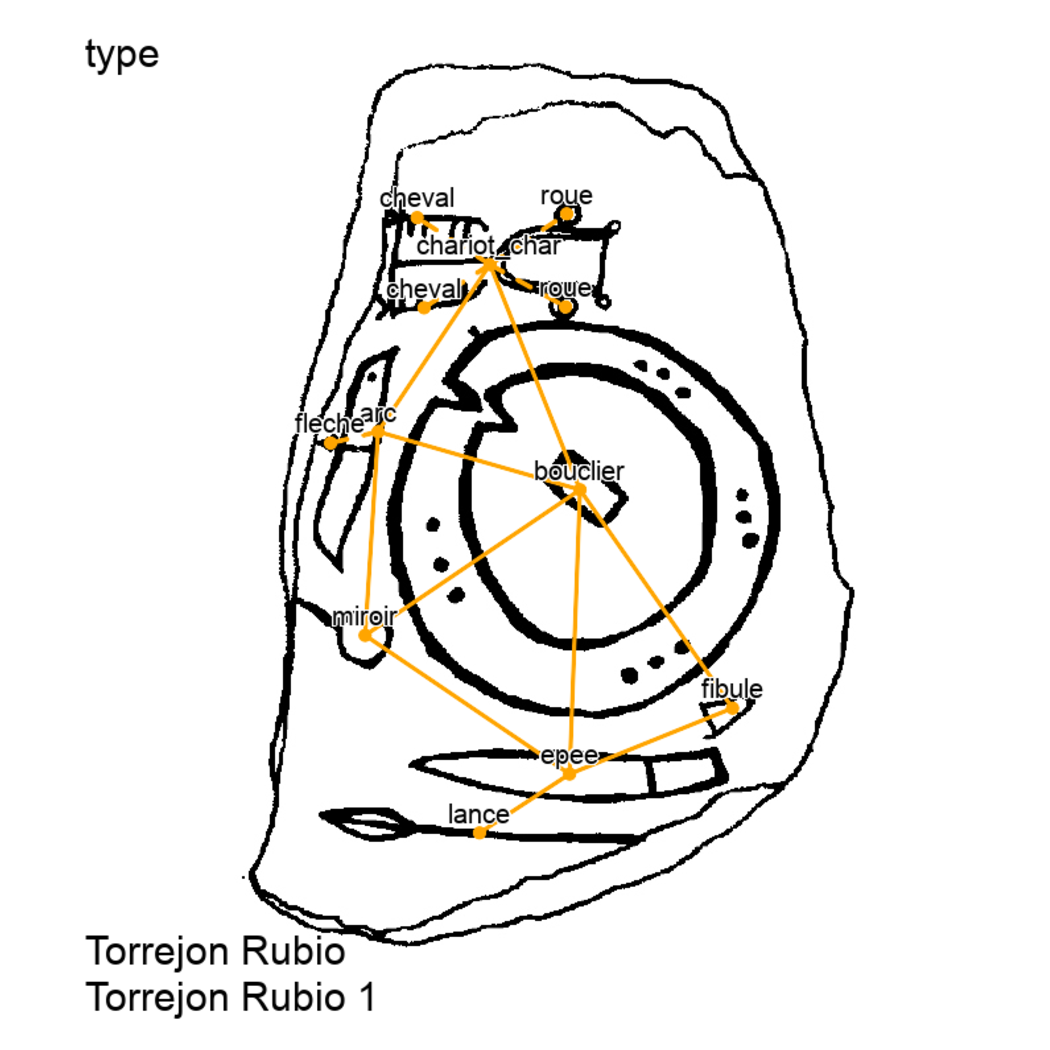
\includegraphics[width=\maxwidth]{figure/plotcm-1} 

\end{knitrout}
\captionof{figure}[directional links]{\emph{Torrejon Rubio 1}}
\end{figure}

\subsection{Decoration comparisons function} \label{sec:functions_one}

The functions allowing to compare different decorations with geometric graphs are

\begin{itemize}
  \item \code{list_nds_compar()} and \code{list_eds_compar()} functions allow to compare respectively the common nodes and the common edges between two decorations
\end{itemize}

Comparisons between pairwise of decorations are first stored into list. These comparisons are performed for nodes and/or edges. There are four (4) decorations in the default dataset, so there is $\frac{4!}{(4-2)!2!}={6}$ pairwise comparisons

% latex table generated in R 3.6.1 by xtable 1.8-4 package
% Thu Sep 24 12:13:42 2020
\begin{table}[ht]
\centering
\begin{tabular}{rll}
  \hline
 & decorA & decorB \\ 
  \hline
1 & Cerro Muriano 1 & Torrejon Rubio 1 \\ 
  2 & Cerro Muriano 1 & Brozas \\ 
  3 & Cerro Muriano 1 & Zarza De Montanchez \\ 
  4 & Torrejon Rubio 1 & Brozas \\ 
  5 & Torrejon Rubio 1 & Zarza De Montanchez \\ 
  6 & Brozas & Zarza De Montanchez \\ 
   \hline
\end{tabular}
\caption{comparison dataframe} 
\label{Test_table_1}
\end{table}



\begin{itemize}  
  \item \code{plot_nds_compar()} and \code{plot_eds_compar()} functions allow to plot and save two figures side-by-side for a decorations pairwise with, respectively, common nodes and common edges identified
\end{itemize}

The \code{plot_nds_compar()}and \code{plot_eds_compar()} functions create a \code{.png} image of two decorations plotted side-by-side with common nodes or edges identified. Functions returns also the name of the image. The common edges or nodes are displayed in red by default. Let us choose the decorations \code{1} (\emph{Cerro Muriano 1}) and \code{4} (\emph{Zarza de Montsanchez})

\begin{figure}[H]
\SweaveOpts{width=20,height=10}
\begin{knitrout}
\definecolor{shadecolor}{rgb}{0.969, 0.969, 0.969}\color{fgcolor}\begin{kframe}
\begin{alltt}
\hlkwd{par}\hlstd{(}\hlkwc{mar}\hlstd{=}\hlkwd{c}\hlstd{(}\hlnum{0}\hlstd{,}\hlnum{0}\hlstd{,}\hlnum{0}\hlstd{,}\hlnum{0}\hlstd{))}
\hlstd{eds_compar} \hlkwb{<-} \hlkwd{plot_eds_compar}\hlstd{(g.compar,} \hlkwd{c}\hlstd{(}\hlnum{1}\hlstd{,}\hlnum{4}\hlstd{),}
                              \hlkwc{doss} \hlstd{=} \hlkwd{system.file}\hlstd{(}\hlstr{"extdata"}\hlstd{,} \hlkwc{package} \hlstd{=} \hlstr{"decorr"}\hlstd{))}
\hlkwd{plot}\hlstd{(}\hlkwd{image_read}\hlstd{(eds_compar))}
\end{alltt}
\end{kframe}
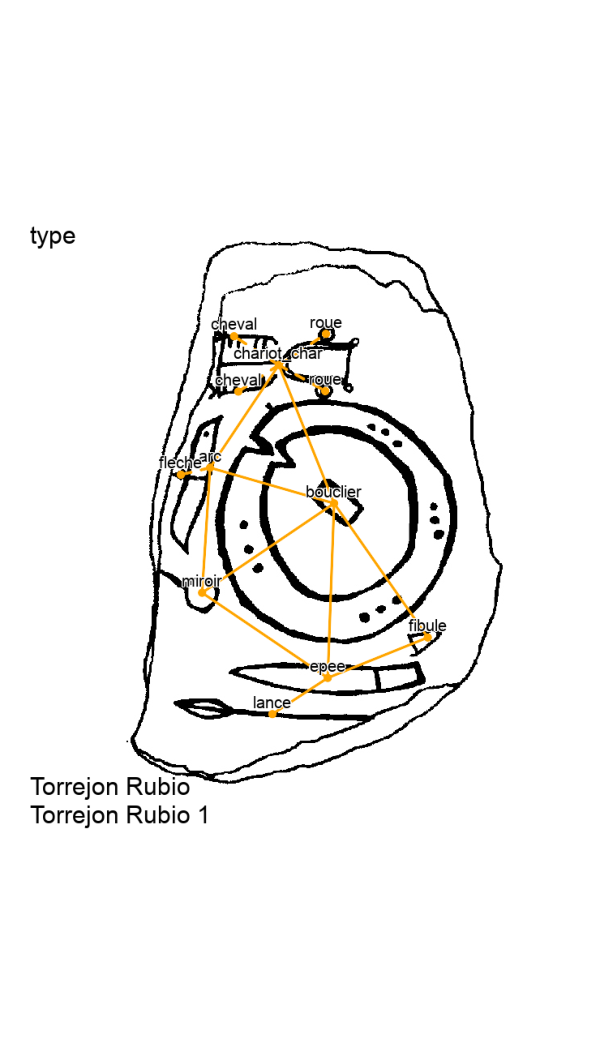
\includegraphics[width=\maxwidth]{figure/unnamed-chunk-11-1} 

\end{knitrout}
\captionof{figure}[directional links]{comparisons between \code{1} (\emph{Cerro Muriano 1}) and \code{4} (\emph{Zarza de Montsanchez} decorations}
\label{edg_comp}
\end{figure}

The comparison on Figure \ref{edg_comp} shows that \code{1} (\emph{Cerro Muriano 1}) and \code{4} (\emph{Zarza de Montsanchez} decorations have two (2) common edges: \texttt{lance -=- personnage} and \texttt{bouclier -=- personnage}


\begin{itemize}
  \item \code{same_nds()} and \code{same_eds()} functions allow to repectively count matching nodes and matching edges between decoration pairwises
\end{itemize}

\code{same_nds()} and \code{same_eds()} allow to repectively count matching nodes and matching edges between decoration pairwises. The result is a square matrix with all pairwise comparisons and the number of common nodes or edges in the cells.

\begin{kframe}
\begin{alltt}
\hlstd{df.same_edges} \hlkwb{<-} \hlkwd{same_eds}\hlstd{(lgrph,}\hlstr{"type"}\hlstd{)}
\hlstd{caption} \hlkwb{<-} \hlstr{"Number of same edges between all decoration pairwise comparisons"}
\hlkwd{print}\hlstd{(xtable}\hlopt{::}\hlkwd{xtable}\hlstd{(df.same_edges,}
                     \hlkwc{caption}\hlstd{=caption,}
                     \hlkwc{label}\hlstd{=}\hlstr{"Test_table_2"}\hlstd{,}
                     \hlkwc{size}\hlstd{=}\hlnum{8}\hlstd{,}
                     \hlkwc{digits}\hlstd{=}\hlkwd{c}\hlstd{(}\hlnum{0}\hlstd{)),}
      \hlkwc{include.rownames}\hlstd{=}\hlnum{TRUE}\hlstd{)}
\end{alltt}
\end{kframe}% latex table generated in R 3.6.1 by xtable 1.8-4 package
% Thu Sep 24 12:13:43 2020
\begin{table}[ht]
\centering
\begin{tabular}{rrrrr}
  \hline
 & 1 & 2 & 3 & 4 \\ 
  \hline
1 & 0 & 0 & 1 & 2 \\ 
  2 & 0 & 0 & 3 & 7 \\ 
  3 & 1 & 3 & 0 & 1 \\ 
  4 & 2 & 7 & 1 & 0 \\ 
   \hline
\end{tabular}
\caption{Number of same edges between all decoration pairwise comparisons} 
\label{Test_table_2}
\end{table}


For these two last exemples, the edges comparisons between the decoration \code{1} and the decoration \code{4} show that they have two (2) common edges.


\section{Illustrations} \label{sec:illustrations}

In order to demonstrate the first insight of a graph-based analysis of the decorations, we will compare two classifications, one based on the presence of common nodes, the second based on the presence of common edges. As said, the first method (presence of common nodes) is the most commonly used method in statistical analysis on decorations since the exact location of the GUs is not commonly registred

\begin{table}[htb]
\begin{minipage}{.45\textwidth}
\centering
% latex table generated in R 3.6.1 by xtable 1.8-4 package
% Thu Sep 24 12:13:43 2020
\begin{tabular}{rrrrr}
  & 1 & 2 & 3 & 4 \\ 
 1 & 0 & 2 & 3 & 4 \\ 
  2 & 2 & 0 & 5 & 7 \\ 
  3 & 3 & 5 & 0 & 4 \\ 
  4 & 4 & 7 & 4 & 0 \\ 
  \end{tabular}

\captionof{table}{Common nodes table}
\end{minipage}
\begin{minipage}{.45\textwidth}
\centering
% latex table generated in R 3.6.1 by xtable 1.8-4 package
% Thu Sep 24 12:13:43 2020
\begin{tabular}{rrrrr}
  & 1 & 2 & 3 & 4 \\ 
 1 & 0 & 0 & 1 & 2 \\ 
  2 & 0 & 0 & 3 & 7 \\ 
  3 & 1 & 3 & 0 & 1 \\ 
  4 & 2 & 7 & 1 & 0 \\ 
  \end{tabular}

\captionof{table}{Common edges table}
\end{minipage}
\end{table}

\begin{figure}[H]
\begin{knitrout}
\definecolor{shadecolor}{rgb}{0.969, 0.969, 0.969}\color{fgcolor}\begin{kframe}
\begin{alltt}
\hlkwd{library}\hlstd{(matlib)}
\end{alltt}


{\ttfamily\noindent\color{warningcolor}{\#\# Warning: package 'matlib' was built under R version 3.6.3}}\begin{alltt}
\hlkwd{par}\hlstd{(}\hlkwc{mfrow}\hlstd{=}\hlkwd{c}\hlstd{(}\hlnum{1}\hlstd{,}\hlnum{2}\hlstd{))}
\hlstd{dist.nodes}  \hlkwb{<-} \hlkwd{dist}\hlstd{(}\hlkwd{inv}\hlstd{(}\hlkwd{as.matrix}\hlstd{(df.same_nodes)))}
\hlstd{dist.edges}  \hlkwb{<-} \hlkwd{dist}\hlstd{(}\hlkwd{inv}\hlstd{(}\hlkwd{as.matrix}\hlstd{(df.same_edges)))}
\hlkwd{plot}\hlstd{(}\hlkwd{hclust}\hlstd{(dist.nodes),} \hlkwc{hang} \hlstd{=} \hlopt{-}\hlnum{1}\hlstd{,} \hlkwc{main} \hlstd{=} \hlstr{"common nodes"}\hlstd{)}
\hlkwd{plot}\hlstd{(}\hlkwd{hclust}\hlstd{(dist.edges),} \hlkwc{hang} \hlstd{=} \hlopt{-}\hlnum{1}\hlstd{,} \hlkwc{main} \hlstd{=} \hlstr{"common edges"}\hlstd{)}
\end{alltt}
\end{kframe}
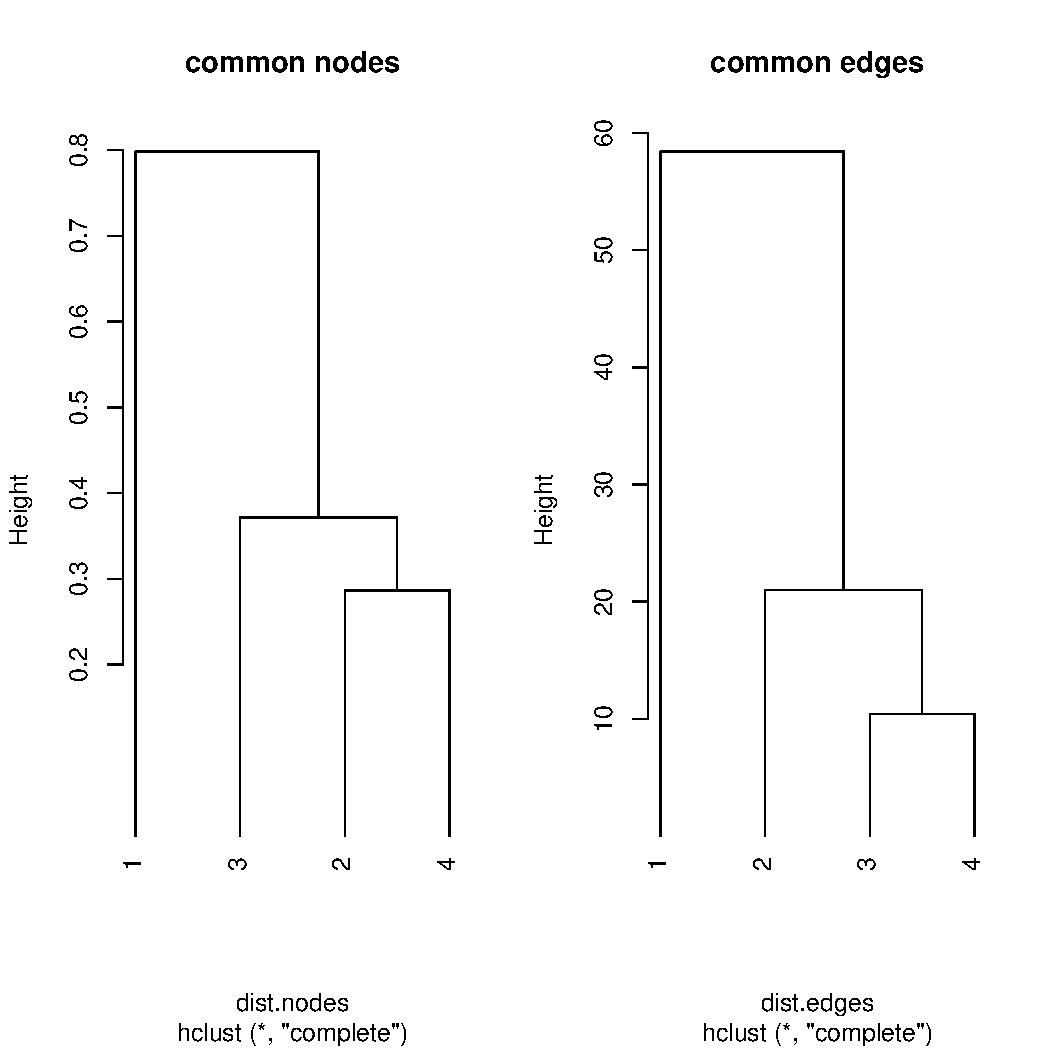
\includegraphics[width=\maxwidth]{figure/unnamed-chunk-15-1} 

\end{knitrout}
\end{figure}

For both nodes and edges, the most distant decorations are \code{1} and \code{4}. These two decorations share four (4) common nodes and, as previously seen, two (2) common edges.
In any cases decorations \code{2} and \code{3} are closer to decoration \code{4} than to decoration \code{1}, but their classifications changes depending on counting of common nodes or common edges. Plotting the comparisons for for \code{3} and \code{4}, helps to understand the differences between the two classifications.

\begin{figure}[H]
\SweaveOpts{width=20,height=20}
\begin{knitrout}
\definecolor{shadecolor}{rgb}{0.969, 0.969, 0.969}\color{fgcolor}
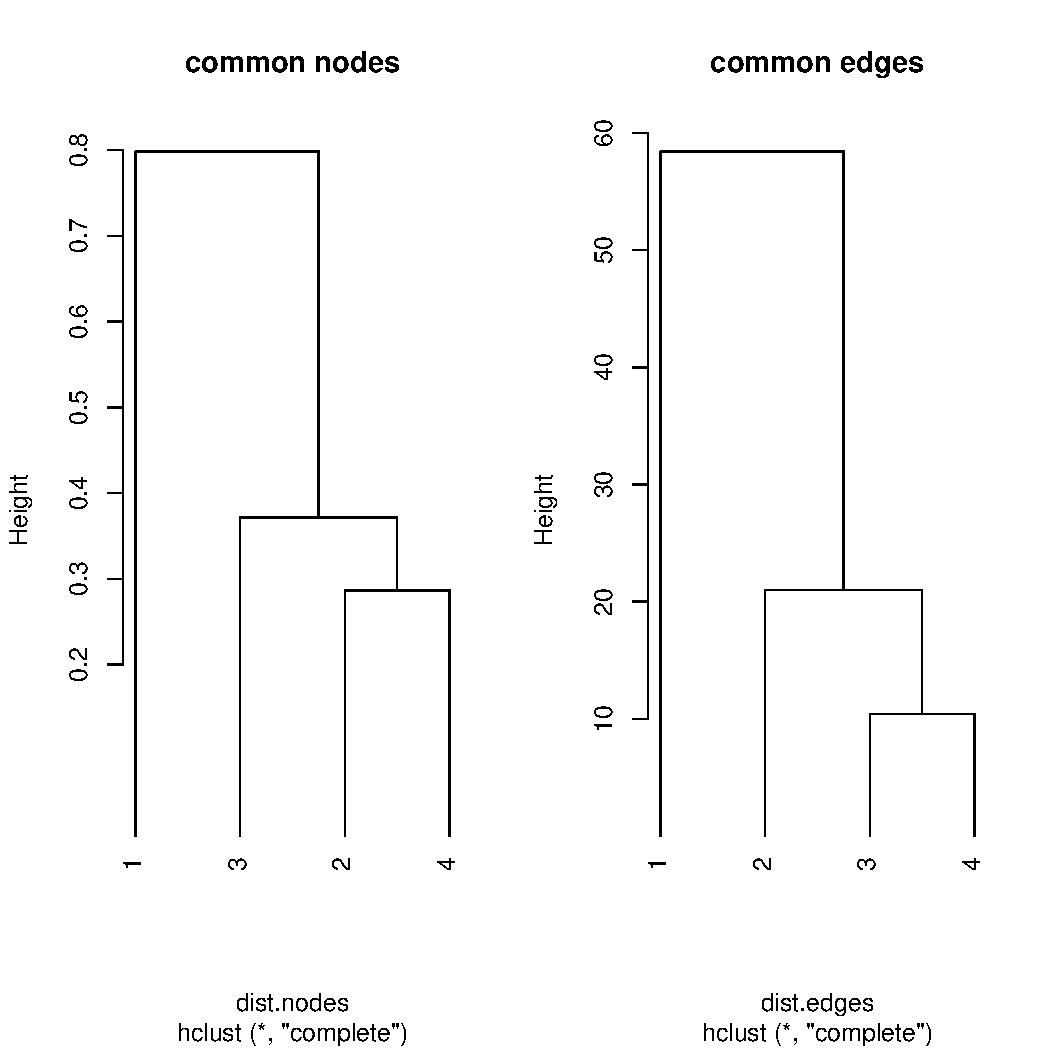
\includegraphics[width=\maxwidth]{figure/unnamed-chunk-16-1} 

\end{knitrout}
\end{figure}


Decorations \code{3} and \code{4} share four (4) common GUs (\code{bouclier, epee, lance, miroir}) but the spatial organisation of theses GUs are different between the two decorations so their number of common edges is lower with only one common edge (\code{bouclier -=- lance})



%% -- Summary/conclusions/discussion -------------------------------------------

\section{Summary and discussion} \label{sec:summary}

\begin{leftbar}
As usual \dots
\end{leftbar}




%% -- Optional special unnumbered sections -------------------------------------

\section*{Computational details}

\begin{leftbar}
If necessary or useful, information about certain computational details
such as version numbers, operating systems, or compilers could be included
in an unnumbered section. Also, auxiliary packages (say, for visualizations,
maps, tables, \dots) that are not cited in the main text can be credited here.
\end{leftbar}

The results in this paper were obtained using
\proglang{R}~3.4.1 with the
\pkg{MASS}~7.3.47 package. \proglang{R} itself
and all packages used are available from the Comprehensive
\proglang{R} Archive Network (CRAN) at
\url{https://CRAN.R-project.org/}.


\section*{Acknowledgments}

\begin{leftbar}
All acknowledgments (note the AE spelling) should be collected in this
unnumbered section before the references. It may contain the usual information
about funding and feedback from colleagues/reviewers/etc. Furthermore,
information such as relative contributions of the authors may be added here
(if any).
\end{leftbar}


%% -- Bibliography -------------------------------------------------------------
%% - References need to be provided in a .bib BibTeX database.
%% - All references should be made with \cite, \citet, \citep, \citealp etc.
%%   (and never hard-coded). See the FAQ for details.
%% - JSS-specific markup (\proglang, \pkg, \code) should be used in the .bib.
%% - Titles in the .bib should be in title case.
%% - DOIs should be included where available.

\bibliography{D:/DocumentationArcheo/biblio10}


%% -- Appendix (if any) --------------------------------------------------------
%% - After the bibliography with page break.
%% - With proper section titles and _not_ just "Appendix".

\newpage

\begin{appendix}

\section{More technical details} \label{app:technical}

\begin{leftbar}
Appendices can be included after the bibliography (with a page break). Each
section within the appendix should have a proper section title (rather than
just \emph{Appendix}).

For more technical style details, please check out JSS's style FAQ at
\url{https://www.jstatsoft.org/pages/view/style#frequently-asked-questions}
which includes the following topics:
\begin{itemize}
  \item Title vs.\ sentence case.
  \item Graphics formatting.
  \item Naming conventions.
  \item Turning JSS manuscripts into \proglang{R} package vignettes.
  \item Trouble shooting.
  \item Many other potentially helpful details\dots
\end{itemize}
\end{leftbar}


\section[Using BibTeX]{Using \textsc{Bib}{\TeX}} \label{app:bibtex}

\begin{leftbar}
References need to be provided in a \textsc{Bib}{\TeX} file (\code{.bib}). All
references should be made with \verb|\cite|, \verb|\citet|, \verb|\citep|,
\verb|\citealp| etc.\ (and never hard-coded). This commands yield different
formats of author-year citations and allow to include additional details (e.g.,
pages, chapters, \dots) in brackets. In case you are not familiar with these
commands see the JSS style FAQ for details.

Cleaning up \textsc{Bib}{\TeX} files is a somewhat tedious task -- especially
when acquiring the entries automatically from mixed online sources. However,
it is important that informations are complete and presented in a consistent
style to avoid confusions. JSS requires the following format.
\begin{itemize}
  \item JSS-specific markup (\verb|\proglang|, \verb|\pkg|, \verb|\code|) should
    be used in the references.
  \item Titles should be in title case.
  \item Journal titles should not be abbreviated and in title case.
  \item DOIs should be included where available.
  \item Software should be properly cited as well. For \proglang{R} packages
    \code{citation("pkgname")} typically provides a good starting point.
\end{itemize}
\end{leftbar}

\end{appendix}

%% -----------------------------------------------------------------------------


\end{document}
